%\newpage
%$ $
%\newpage

\renewcommand{\thesubsection}{\textcolor{red}{\Roman{section}.\arabic{subsection}}}
\renewcommand{\thesubsubsection}{\textcolor{red}{\Roman{section}.\arabic{subsection}.\alph{subsubsection}}}

\setcounter{section}{0}
\setcounter{document}{0}
\sndEnTeteTPTrois

\begin{center}
\begin{mdframed}[style=titr, leftmargin=60pt, rightmargin=60pt, innertopmargin=7pt, innerbottommargin=7pt, innerrightmargin=8pt, innerleftmargin=8pt]

\begin{center}
\large{\textbf{TP 3 : Détermination de la composition d'un mélange : l'alcool pharmaceutique}}
\end{center}

\end{mdframed}
\end{center}



\begin{tcolorbox}[colback=blue!5!white,colframe=blue!75!black,title=Objectifs de la séance :]
Mesurer des volumes et des masses pour estimer la composition de mélanges.
\end{tcolorbox}

\begin{tcolorbox}[colback=orange!5!white,colframe=orange!75!black,title= Scénario:]
Un pharmacien vend de l’alcool pharmaceutique (mélange eau-éthanol), qui sert de désinfectant notamment pour le matériel médical. L’étiquette d’un flacon d’alcool pharmaceutique porte la mention de sa composition. Le pharmacien aimerait s’assurer que cette indication est correcte.
\end{tcolorbox}

\section{Documents mis à disposition}

\begin{multicols}{2}
    \begin{doc}{Flacon d'alcool pharmaceutique}
\begin{center}
    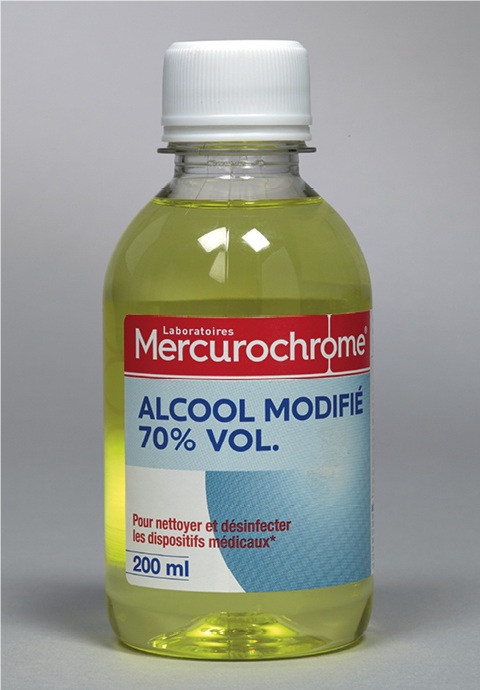
\includegraphics[scale=0.81]{Images/TP3/Alcool_pharma.png}
\end{center}
\end{doc}
\begin{doc}{Variation de la masse volumique d’un mélange eau-éthanol en fonction du pourcentage volumique en éthanol}
\vspace{-1cm}
\begin{center}
    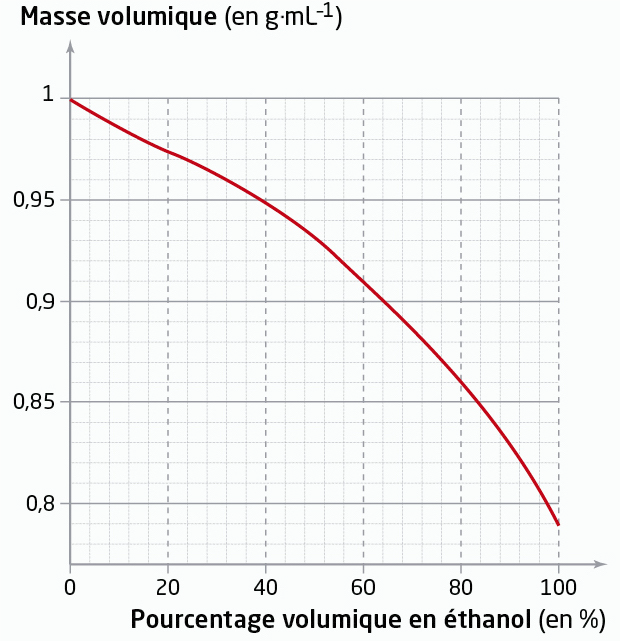
\includegraphics[scale=0.75]{Images/TP3/Masse_vol_ethanol.png}
\end{center}
\end{doc}

\end{multicols}

\newpage

\begin{mdframed}[style=autreexo]
\textbf{\bsc{Liste du matériel}}
\begin{itemize}
    \item un flacon contenant de l'alcool pharmaceutique
    \item une balance
    \item une éprouvette graduée de 10mL
    \item une fiole jaugée de 25mL
    \item une pissette en plastique
    \item un bécher de 25mL 
\end{itemize}
\end{mdframed}


\section{Travail à effectuer}

\question{À l’aide du document 2, déterminer la masse volumique de l’éthanol pur, ainsi que la masse volumique de l’eau.}{Par lecture graphique, on lit $\rho_{eau}=1$~g.mL$^{-1}$ lorsque le pourcentage volumique en éthanol est égal à 0\% et $\rho_{ethanol}=0.79$~g.mL$^{-1}$ lorsque le pourcentage volumique en éthanol est égal à 100\%.}{0}

\question{Proposer un protocole permettant de déterminer expérimentalement la masse volumique de l’alcool pharmaceutique vendu par le pharmacien.}{On pèse la verrerie qu'on va utiliser (bécher, fiole jaugée ou éprouvette graduée). On tare la balance (ou on note la masse de la verrerie pour la soustraire par la suite). On verse un volume V d'alcool pharmaceutique dans la verrerie en s'aidant des traits de graduation de la verrerie. On vérifie que le bas du ménisque coïncide bien avec la graduation. On note le volume versé $V$. On pèse ensuite l'ensemble \{verrerie+alcool\} pour en déduire la masse d'alcool versé.}{0}

\question{Appeler le porfesseur pour valider votre protocole expérimental.}{}{0}

\question{Mettre en \oe uvre le protocole précédent et déterminer la masse volumique de l’alcool pharmaceutique vendu par le pharmacien.}{On pèse l'éprouvette graduée à vide, on remplit d'un certain volume d'alcool pharmaceutique $V$ et on pèse l'ensemble. On en déduit la masse volumique $\rho=\frac{m_{verrerie+eau/ethanol}-m_{verrerie}}{V}$
. On laisse ici le choix de la verrerie, le TP suivant permettra d'appréhender la précision des différents types de verrerie. Mais pour une mesure précise, il faut choisir ici une fiole jaugée.}{0}

\question{La législation autorise un écart de $\pm~2\%$.VOL sur la proportion volumique d'éthanol contenue dans ce produit. Déterminer si l’indication portée sur le flacon d’alcool pharmaceutique vendu est conforme.}{La mesure doit être conforme à la valeur indiquée. Si l'écart entre la mesure et la valeur indiquée est supérieur à 2\%, on peut mettre en cause :
\begin{itemize}
    \item le choix de la verrerie dans le protocole : effectivement, si le choix s'est porté sur le bécher, le volume lu est peu précis (5\% sur la valeur lue au moins),
    \item la quantité réelle d'éthanol contenue : l'éthanol étant volatil, une petite quantité a pu s'évaporer du flacon modifiant la masse volumique du mélange.
\end{itemize}}{0}

\question{L’alcool pharmaceutique vendu par le pharmacien a été préparé en utilisant 75 mL d’eau. Calculer le volume d’éthanol qu’il a fallu ajouter pour fabriquer cet alcool.}{On sait que la proportion volumique en éthanol vaut $x_V=\frac{V_{ethanol}}{V_tot}=70$\%. Comme $V_{tot}=V_{ethanol}+V_{eau}$, on en déduit : 
\begin{align*}
    \frac{V_{ethanol}}{V_{ethanol}+V_{eau}} &= 0,70 \\
    V_{ethanol} &= 0,70\times (V_{ethanol}+V_{eau}) \\
    V_{ethanol}\times (1-0,70) &= V_{eau} \\
    V_{ethanol}  &= \frac{V_{eau}}{1-0,70} = \frac{75~\text{mL}}{1-0,70}=250~\text{mL}
\end{align*}}{0}